\chapter{Test}
Development of any electronic system involves many different stages which finally lead to manufacturing process and later on to the use phase of such a system. At every stage of its life cycle the system has to be tested for presence of faults. This process doesn't have to end with a post-manufacturing test. As shown in the previous chapter, the faults accompany the system from the very first ideas of its developers until its final power down. The \autoref{fig:design} shows the following design stages with accompanying tests.

\begin  {figure}  [H]
\centering
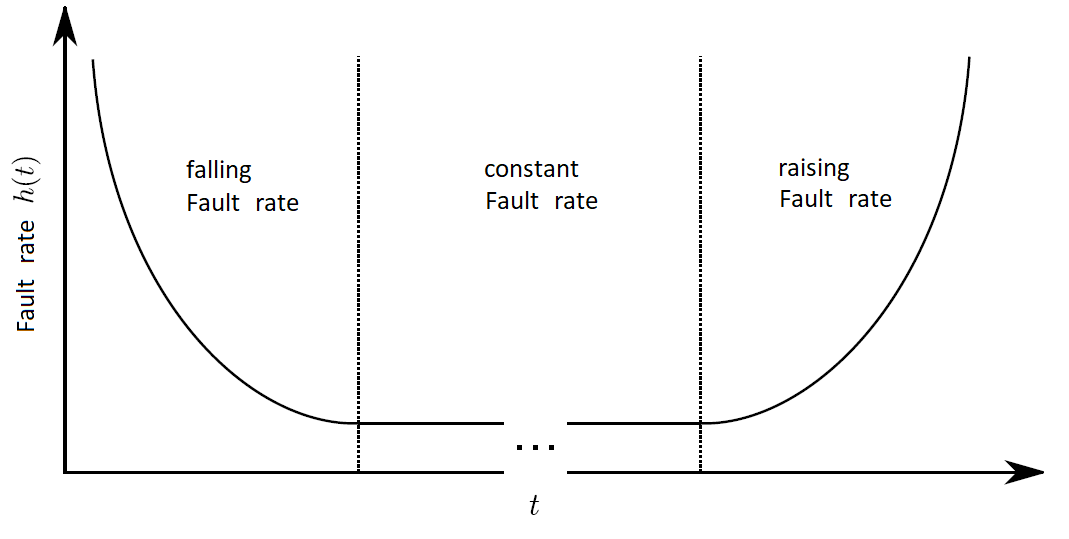
\includegraphics[width=0.65\textwidth]{figures/badewanne.png}
\caption{Fault rate throughout systems life cycle~\cite{art:Avizienis}}
\label{fig:badewanne}
\end {figure}

\section{Fault models}

The amount of different faults and their variety is countless. There are means needed to model how those faults affect the system. The fault effects are called failure modes. There is no perfect model that would cover all faults but there are specific failure modes that can be observed and are common to many different faults, like following:
\begin{itemize}
    \item Single Event Transient (SET) describes a glitch in combinational logic that travels trough design
    \item Single Event Upset (SEU) describes the situation when the incorrect voltage level caused by SET gets stored in the memory or the memory state changes. Can affect more memory cells at once.
    \item Single Event Latchup (SEL) - a highly loaded particle makes a locked transistor conduct leading to short in CMOS logic. Requires a power reset and may lead to a hard fault, because of a very high temperature~\cite{report:altera}.
\end{itemize}
The abstraction of faults and categorization into failure modes allows to develop test methods to simulate this particular effect. All mentioned models represent failure modes in digital hardware logic. Some operations take less time or energy when moved from digital domain to analog one~\cite{Prof Vierhaus Lectures}. In modern communication systems there is a rapid growth in analog and mixed circuitry that is also vulnerable to faults. The number of such faults is again countless and some failure mode representation is needed. The continuous characteristic of analog systems allows only for two failure modes:
\begin{itemize}
    \item Catastrophic failures - the system is not functional at all
    \item Unacceptable performance - the service is still provided but some of the functionality lies outside of the acceptable range of the specification
\end{itemize}
The distinction between them lies only in the definition of catastrophic failure and definition range of the system. On higher abstraction levels the catastrophic fault may only be considered as a parametric one~\cite{book:Kabisatpathy}, following the rule of fault propagation mentioned in~\autoref{fig:propagation}.

%diagnostic test
%online offline testing
% DFT, scan path, boundry scna, BIST
